\documentclass[12pt,a4paper,onecolumn]{article}
\usepackage[utf8]{inputenc}

\usepackage[english]{babel}

\usepackage{quoting}

\usepackage{caption}

\usepackage{graphicx}

\usepackage{fancyvrb}

\usepackage{float}

\usepackage{tikz}

\usepackage{cancel}

\usepackage{subfigure}
\parindent=5mm                        
\parskip=3mm 
\usepackage[left=1.75cm,right=1.75cm,top=2cm,bottom=3cm]{geometry}

\usepackage{amsfonts}  % required for math formulae
\usepackage{amsmath}   % required for math formulae
\usepackage[T1]{fontenc}
% \usepackage[cp1250]{inputenc}
\graphicspath{ {./Figures/} }

\setlength{\parindent}{0pt}   % no indent at the beginning of paragraphs
\setlength{\parskip}{2.5ex}   % space between the paragraphs

%\linespread{1.5}

\pagenumbering{arabic}

\usepackage{hyperref}

\hypersetup{
    colorlinks=true,
    linkcolor=blue,
    filecolor=magenta,      
    urlcolor=cyan,
}

%pacchetti
\usepackage{quoting}
\usepackage{booktabs}
\usepackage{array}
\usepackage{amsthm} 
\usepackage{amssymb}
\usepackage{mathtools}
\usepackage{braket}
\usepackage{empheq}
\usepackage{fancyvrb}
\usepackage{frontespizio}

%definizioni e teoremi
\theoremstyle{definition}
\newtheorem*{definizione}{Definizione}
\theoremstyle{plain}
\newtheorem*{teorema}{Teorema}

%Macro for \var
 \newcommand{\var}{\varphi} 

%matematica
\newcommand{\numberset}{\mathbb}
\newcommand{\N}{\numberset{N}}
\newcommand{\R}{\numberset{R}}
\newcommand{\Z}{\numberset{Z}}
\newcommand{\Q}{\numberset{Q}}
\newcommand{\C}{\numberset{C}}
\renewcommand{\epsilon}{\varepsilon}
%\renewcommand{\rho}{\varrho}
\renewcommand{\phi}{\varphi}
\DeclarePairedDelimiter{\abs}{\lvert}{\rvert}
\DeclarePairedDelimiter{\norma}{\lVert}{\rVert}
%%%%%%


% title page begins here
\thispagestyle{empty} % title page with no number

\begin{document}




\includegraphics[scale=0.4]{ecmi-logo}

ECMI Modeling Week 2019\\
University of Grenoble - Grenoble INP

\begin{center}
\vspace{2.0cm}
{\Large{\textbf{Detection of resonances for the modelling of resonant tunneling devices}}}

\vspace{\stretch{0.01}}

Instructor: Clément Jourdana - University of Grenoble Alpes
\vspace{\stretch{0.01}}

\begin{tabular}{rl}
S. Baltieri & (Università degli studi di Verona ) \\
A. Carballosa & (Universidad Autónoma de Barcelona) \\
M. Feder & (Università degli studi di Verona) \\
A. Tonini & (Università degli studi di Milano) \\
M. Zarcheva & (Sofia University, "St. Kliment Ohridski")
\end{tabular}

\vspace{\stretch{0.5}}

%Date of the report
05.09.2019
\end{center}

\vspace{\stretch{0.15}}




\newpage

\tableofcontents

\newpage

\section{Introduction}
In Quantum mechanics, the simplest unidimensional problems are the cases for a potential form of a barrier and a well, illustrated in Figure \ref {fig:1Dproblems}. For each one of these problems, one unique phenomenon occurs that is only observed in the quantum realm. In the first case, when one particle faces a potential barrier with energy lower than the height of the barrier, in the classical point of view, the particle will be reflected assuming that the impact with the barrier preserves energy and momentum. However, in quantum mechanics, the particle has a non-zero probability to appear on the other side of the barrier, since the particle does not have now a deterministic trajectory, but a density of probability of being at position $x$ and time $t$ distributed across a determined region of space. In this sense, the particles propagates in space according to a wave function $\psi$ and when encountering the barrier will have a probability of being reflected and a probability of being transmitted. The latter is measured through the transmission coefficient, and the probability density in each region of the space can be computed from the Schrödinger equation (in 1D), introducing the appropiate initial and boundary conditions to account for the potential: 

\begin{align}
    -\frac{\hbar^2}{2m}\frac{\partial^2\psi(x,t)}{\partial x^2 }&+V(x)\psi(x,t)=i\hbar \frac{\partial \psi(x,t)}{\partial t} \\
    &V(x)=
\begin{cases}
V_0\hspace{1cm} \text{if } a<x<b\\
0\hspace{1cm} \text{elsewhere}
\end{cases}
\end{align}

\begin{figure}[h!]
\centering
		\subfigure[]{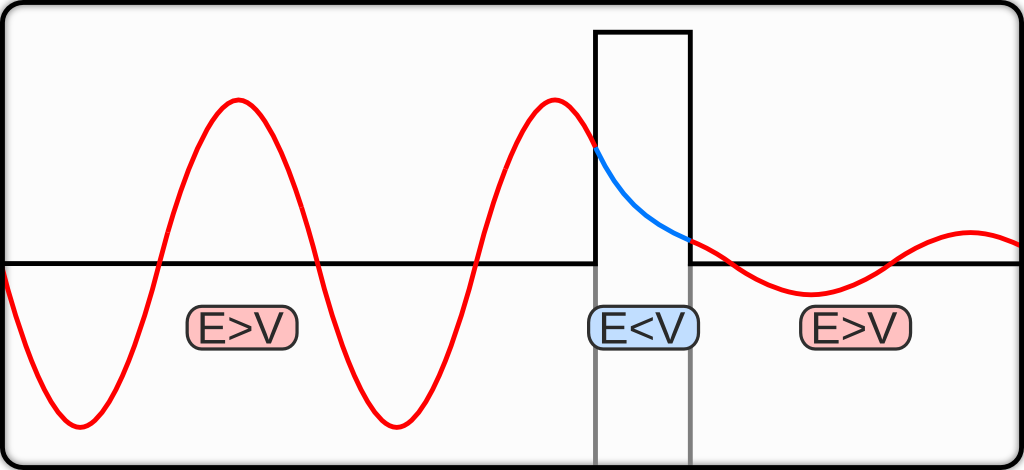
\includegraphics[width=0.45\linewidth]{tunneling.png}}
		\subfigure[]{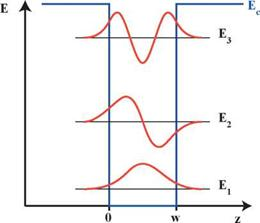
\includegraphics[width=0.35\linewidth]{quantum_well.jpg}}
	\caption{Quantum tunneling through a potential barrier (fig a)) and a potential well with its discrete energy levels (fig b)). Figures extracted from {\url{http://elektroarsenal.net/quantum-wells.html}} and {\url{https://brilliant.org/wiki/quantum-tunneling/}} }
	\label{fig:1Dproblems}
\end{figure}

In the problem of one particle enclosed in the quantum well, by solving Schröedinger equation one finds that the energy states of the particle are discretized as Figure \ref {fig:1Dproblems} shows, instead of the continuous range that one would expect in classical dynamics. 

Now, here what concerns us is the interesting problem of putting together two or more potential barriers creating a quantum well in the middle. This is what occurs in the resonant tunneling devices, which receive its name because it is observed that for some incident energy of the electrons the transmission coefficient equals the unity. This is, the electrons go through the device without "seeing" the barriers. The nature of this curious effect arises from the discretization of the energy states inside the quantum well, producing that when the energy of the incident electron coincides with one of the energy levels of the well, the transmission coefficient peaks to one, as shown in Figure \ref {fig:2barriers_problem}. This effect allows for an application of resonant tunneling transistors as promising switching devices, ideal for memory storing. 

\begin{figure}[h!]
\centering
		\subfigure[]{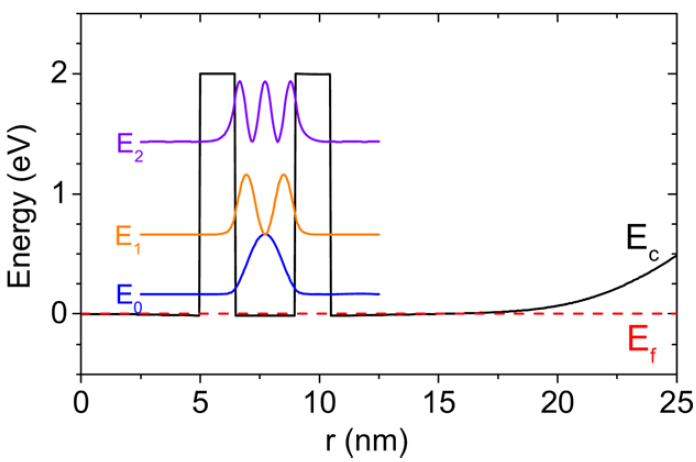
\includegraphics[width=0.48\linewidth]{double_barrier.png}}
		\subfigure[]{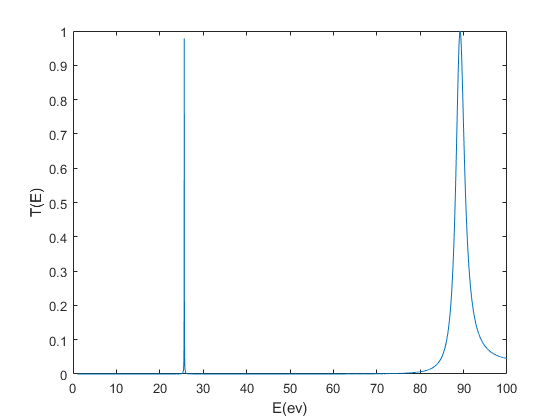
\includegraphics[width=0.45\linewidth]{tE.png}}
	\caption{Resonant tunneling (fig a)) and transmission coefficient (fig b)) for a double barrier. Fig. a) was extracted from {\url{http://dx.doi.org/10.1063/1.3701586}}} 
	\label{fig:2barriers_problem}
\end{figure}

In this work, we attempt to study the problem of two or more potential barriers from a numerical point of view and in an ideal situation (with null potential difference between the extremities of the device). For this purpose, we find that the main feature of the problem is to characterize accurately the transmission coefficient in function of the incident energy, since this curve will provide all the information needed on the energy resonances and the transmission peaks. Considering that each value of the energy will imply solving one time the Schröedinger equation, we must also find a strong optimization to the numerical implementation in order to reduce the computational work, solving therefore a more reasonable number of differential equations. The optimization that we will describe here will be that of an adaptive mesh scheme in the energy discretization.

\section{Preliminary computations}
\subsection{Finding the transmission coefficient \textbf{T}}


As a beginning, we  will make a quick review of the process of \textit{quantum tunneling}.

Let us consider a current or voltage wave, travelling through a transmission line from a generating source towards a load. This wave becomes an \textit{incident wave} when it meets a discontinuity or another medium with different propagation characteristics. In this situation, some or all of the wave will be reflected back in the direction of the origin \cite{IncidentWave}.

If a wave travelling within a force field reaches a region that has a potential significantly higher than the potential at the points surrounding it, we observe an incident wave upon a \textit{potential barrier}. On quantum level (observing particles and energies on subatomic scale), it is possible for a particle to pass trough the barrier, without having the potential energy required. This phenomenon is known as \textit{quantum tunnelling}.

The quantity that describes the probability of a particle tunneling through a barrier is the so called \textit{transmission coefficient}. By definition, the \textit{transmission coefficient T} is described by the following ratio:
\begin{equation*}
        T=\frac{J_{trans}.\overline{n}}{J_{inj}.\overline{n}},
\end{equation*}
where $J_{inj}$ is the \textit{probability current} in the wave incident upon the barrier with normal unit vector $\overline{n}$, and $J_{trans}$ is the \textit{probability current} in the wave that has passed on the other side of the barrier \cite{wikiTransmCoeff}.

In the following section, we will introduce the concept of \textit{probability current}.


\subsection{The probability current}
Probability current (probability flux) is a formalism in quantum mechanics that describes the flow of probability. It is defined as the probability per unit time, per unit area. 
We need to establish a connection between the variables in the model and the unknown probability flux in order to compute the transmission coefficient $T$.

It is not a coincidence that the quantity of interest is called probability \textit{flux}. When talking about flux, the first thing to come in mind is the continuity equation. It appears that there is a conserved quantity in the process, that is, the \textit{probability density} and we can obtain the definition of probability flux, using it \cite{ConservationLaw}. If one thinks about the \textit{probability density} as a heterogeneous fluid, then the \textit{probability current} is the rate of flow of this fluid \cite{wikiProbCurrent}. \\
The \textit{probability density} is defined as
    \begin{equation*}
    P(x,t) = |\psi|^2=\psi^{*}(x,t) \psi(x,t),
    \end{equation*}
    where $\psi^{*}$ is the complex conjugate of $\psi$.\\ \\
    Differentiating it with respect to time, we obtain
    \begin{equation} \label{prob_density_eq}
    \frac{\partial}{\partial t} P(x,t) =
    \left[\frac{\partial \psi^{*}}{\partial  t} \psi +
    \psi^{*} \frac{\partial \psi}{\partial  t} 
    \right].
    \end{equation}
    
    Using the $Shr\ddot{o}dinger$ equaiton for $\psi$ and its complex conjugate, multiplying them for $\psi^{*}$ and $\psi$ respectively, and replacing them in \eqref{prob_density_eq}, we arrive at

\begin{align*}
        \psi^{*}\left(\textbf{i} \hbar \frac{\partial \psi}{\partial t}\right) &= \left(-\frac{\hbar^2}{2m} \frac{\partial^2 \psi}{\partial x^2} + V(x)\psi\right)\psi^{*}\\ \\
        \psi \left(-\textbf{i} \hbar \frac{\partial \psi^{*}}{\partial t}\right) &= \left(-\frac{\hbar^2}{2m} \frac{\partial^2 \psi^{*}}{\partial x^2} + V(x)\psi^{*}\right)\psi
    \end{align*}
  
    \begin{align*}
            \frac{\partial}{\partial t} P(x,t)= &
            \frac{1}{\textbf{i} \hbar}\left[
    \frac{\hbar^2}{2m} \frac{\partial^2 \psi^{*}}{\partial x^2} \psi - \cancel {V(x) \psi^{*}\psi} - 
    \frac{\hbar^2}{2m} \frac{\partial^2 \psi}{\partial x^2} \psi^{*} + 
    \cancel{V(x) \psi^{*} \psi}
    \right] \\
    =&\frac{\hbar}{2m\textbf{i}} \frac{\partial}{\partial x}
    \left[
    \frac{\partial \psi^{*}}{\partial  x} \psi -
    \psi^{*} \frac{\partial \psi}{\partial  x} 
    \right].
    \end{align*}
    
     We define $j(x,t)$ as the \textit{the probability current}:
    \begin{equation}
    \label{definition_of_probability_current}
    j(x,t) =  \frac{\hbar}{2m\textbf{i}}
    \left[
    \psi^{*} \frac{\partial \psi}{\partial  x} -
    \frac{\partial \psi^{*}}{\partial  x} \psi 
    \right]=
    \frac{\hbar}{m}
    Im\left(
    \psi^{*} \frac{\partial \psi}{\partial  x} 
    \right).
    \end{equation}
    
    We have just derived the probability conservation equation
    \begin{equation}
            \frac{\partial P(x,t)}{\partial t} + \frac{\partial j(x,t)}{\partial x} = 0.
    \end{equation}

Now, we can use \eqref{definition_of_probability_current} to compute the transmission coefficient.

\subsection{Time-independent formulation}
The time-dependent $Shr\ddot{o}dinger$ equation predicts that wave functions can form stationary states, called standing waves.
In physics, a standing wave (stationary wave) is a wave which oscillates in time but whose peak amplitude profile does not move in space. The peak amplitude of the wave oscillations at any point in space is constant with time. This phenomenon usually occurs as a result of interference between two waves traveling in opposite directions, for example in the case of resonance \cite{wikiStatState}.

Such stationary state is an eigenvector of the Hamiltonian. This means, that we are observing a situation where the system has a single definite energy (instead of a quantum superposition of different energies). It is also called \textit{energy eigenvector}.

For a single-particle Hamiltonian, a stationary state means that the particle has a constant probability distribution for its position, its velocity, its spin, etc. (this is true assuming that the Hamiltonian is unchanging in time). We should note that the wavefunction itself is not stationary \cite{wikiStatState}.


These states are particularly important as their individual study later simplifies the task of solving the time-dependent $Shr\ddot{o}dinger$ equation for any state. Stationary states can be described by the time-independent $Shr\ddot{o}dinger$ equation. \\

 
The time-independent formulation can be obtained using the classical method of separation of variables, as following\\ \\
Let
\begin{equation*}
    \psi(x,t) = \varphi(x) f(t)
\end{equation*}
\begin{align*}
    &\textbf{i} \hbar  \varphi(x) \frac{d f(t)}{d t} = -\frac{\hbar^2}{2m} \frac{d^2 \varphi(x)}{d x^2} f(t) + V(x)\varphi(x) f(t) \color{gray}{/.\frac{1}{\varphi(x) f(t)}}\\ \\ 
    &\frac{1}{f(t)} \textbf{i} \hbar \frac{d f(t)}{d t} = 
    -\frac{\hbar^2}{2m} \frac{1}{\varphi(x)} \frac{d^2 \varphi(x)}{d x^2} + V(x)=
    const. = E.
\end{align*}\\
 Multiplying by $\varphi(x)$ the space equation\\
\begin{equation}
\label{time-independent-form}
-\frac{\hbar^2}{2m} \frac{d^2 \varphi(x)}{d x^2} = (E-V(x))\varphi(x),
\end{equation}\\
where $E$ is a constant equal to the energy level of the system. \\

\subsection{Nondimesionalization}
Before we start with the numerical computations, what we can notice, is that some very small numbers appear in the main equation. \eqref{SmallNumbers}

\[
\begin{split}
\label{SmallNumbers}
&\frac{\hbar^2}{m}=\frac{(1.054571726\cdot10^{\color{red}{-34}}J s)^{\color{red}{2}}}{9.109383702\cdot 10^{\color{red}{-31}}kg}\approx 1.220852652\cdot 10^{\color{red}{-38}}\frac{J^2 s^2}{kg}\approx 4.756006764\cdot 10^{\color{red}{-1}} \frac{eV^2 s^2}{kg}\\
&1eV = 1.602176634\cdot10^{\color{red}{-19}}J
\end{split}
\]

The length of the domain could be really small (of the order of nanometers). In order to avoid computations with such small numbers, we shall derive a non-dimensional form of the model.
For this purpose, we use the following change of variables:

\begin{equation*}
\overline{x} = \frac{x}{\lambda}\qquad \widetilde{V} = \frac{V(\overline{x})}{E_{c}}\qquad \widetilde{E} = \frac{E(\overline{x})}{E_{c}}
\end{equation*}

\begin{equation*}
    E_{c} := \frac{\hbar^2}{m \lambda^2}\qquad \left[ E_{c} \right] = ML^{-2}T^{-2},
\end{equation*}

with $\lambda$-characteristic length, which is usually set to be the length of the domain of interest, and $E_{c}$ the characteristic energy.\\
Making a substitution in \eqref{time-independent-form}, we obtain
\begin{equation}
\label{non-dim-form}
    \frac{1}{2} \frac{d^2 \varphi}{d \overline{x}^2} = ( \widetilde{V}(\overline{x})-\widetilde{E} ) \varphi(\overline{x})
\end{equation}
From now on, all the experiments in the report are derived using \eqref{non-dim-form}.


\section{Transparent boundary conditions: derivation and assumptions}

Following \cite{bc} we assume that the access zones are $(-\infty,0)$ and $(1, +\infty)$. Those zones are waveguides in which the potential is constant. Then we can solve the Schr{\"o}dinger equation in such regions, and we reduce our problem just to the interval $(0,1)$. The main problem is that we do \emph{not} know the wave function at the new boundaries $x=0$ and $x=1$, therefore the boundary conditions have to be derived from the equation. As we can see from the figure below, the waves can exit the interval  at $x=1$, or be reflected by the potential at $x=0$.

Since access zones are waveguides, we have $V(x)=V(0)=V_0$ for $x <0$ and $V(x)=V(1)=V_1$ for $x>1$ and we can solve the equation explicitely in those regions. 



We have, for $x <0$
\[ 
\varphi(x)=e^{\bold{i}kx}+r(k)e^{-\bold{i}kx} 
\]
\[
\varphi'(x)=\bold{i} k e^{\bold{i}kx} - \bold{i}k r(k)e^{-\bold{i}kx}
\]
where $k  \propto (E-V_0)$, while $r(k)$ is the reflection coefficient. It's easy to see that 
\[ 
\bold{i} k \varphi(0)+\varphi'(0)=[2 \bold{i}k e^{\bold{i}k x} ]_{x=0}=2 \bold{i} k
\]

and this leads to the boundary condition 
\[
 \bold{i} k \var(0)+\var'(0)=2\bold{i}k
 \]

Note that at this point everything is known, even if we do not know explicitly $r(k)$. The very same argument applies to $x=1$ and leads to the boundary condition 
\[ 
\varphi'(1) - \bold{i} k_2\varphi(1)=0
\]

\begin{figure}[h!]
	\centering
	  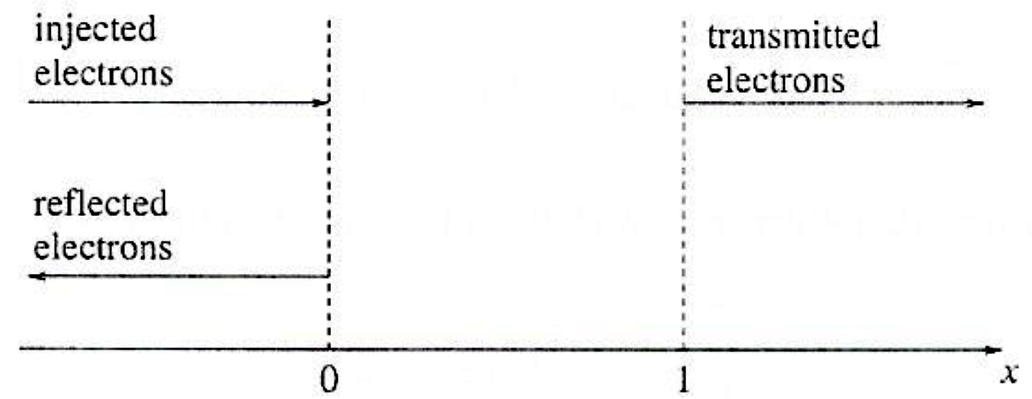
\includegraphics[width=0.8\textwidth]{regions.png}
	  \caption{Electrons are injected at $x=0$ and either reflected ($x=0$) or transmitted at $x=1$}
	  \label{fig:OrderConst}
\end{figure}




\section{A finite difference approximation for Schr{\"o}dinger equation}
\subsection{Finite differences method}
Consider the problem of approximating the derivative of a function $ f $ in an interval $ [a, b] $. A natural way to proceed is to introduce $N$ nodes in $ [a, b] $ $ x_k, k = 1, \dots, N $ with $ x_1 = a $, $ x_N = b $ and $ x_ {k + 1} = x_ {k} + h, k = 1, \dots, N-1 $, where $ h = \frac {b-a} {N-1} $.
Fixed $x_i$, we approximate $f'(x_i)$ with he value of the node $f(x_k)$ in the following way:
\begin{equation}
\label{eqn:somme}
h\sum_{k=-m}^{m}\alpha_{k}u_{i-k} = \sum_{k=-m}^{m} \beta_{k}f(x_{i-k}),
\end{equation}
where $\{\alpha_k\}_{k=-m}^{k=m}, \{\beta_{k}\}_{k=-m}^{k=m} \subseteq \R$.
We note that after setting the coefficients $\{\alpha_i\}$ and $\{\beta_i\}$, to determine the values $u_i$, with $i\in\{1,\dots,N\}$ , it is necessary to solve a linear system. 

In the case of classical finite differences, the intrinsic definition of derivative is used:
\begin{equation}
\label{eqn:derivata}
f'(x_i)= \lim_{h \to 0^{+}}\frac{f(x_i+h)-f(x_i)}{h}.
\end{equation}
By replacing the limit operation with the incremental relationship with $h$ finite, we get the following approximation:
\begin{empheq}{equation}
\label{eqn:cent}
u_i=\frac{f(x_{i+1}) - f(x_{i-1})}{2h}, \quad 2 \le i \le N-1 .
\end{empheq}
The second member of \eqref{eqn:cent} is called \textit{centered finite difference } and corresponds geometrically to have replaced $ f '(x_i) $ with the angular coefficient of the line passing through the points $(x_{i-1},f(x_{i-1}))$ e $(x_{i+1},f(x_{i+1}))$.
Using Taylor series development, we get
\begin{equation}
f'(x_i) - u_i=-\frac{h^2}{6}f'''(\xi_i).
\end{equation}
Then \eqref{eqn:cent} is an approximation of second order with respect to $h$.

\subsection{Finite difference solution of Schr{\"o}dinger equation}

We discretize our domain $\Omega=(a,b)$ with $N$ points and the uniform mesh is made by $N-1$ intervals of length $h=\frac{b-a}{N-1}$.

For the sake of simplicity we consider the nondimensional time independent equation with \emph{transparent boundary conditions}, in $\Omega=(0,1)$, namely


\[ \var''(x)+2(E-V(x))\var(x)=0 \]
 and conditions
 \[ \bold{i} k \var(0)+\var'(0)=2\bold{i}k, \]
 
 \[ \var'(1)=\bold{i} k_2\var(1), \]


where $\bold{i}$ is the imaginary unit and $k_2=\sqrt{k^2+2(V(0)-V(1))}$, $k=\sqrt{2(E-V(0))}$.


Here $V:\mathbb{R} \rightarrow \mathbb{R}$ is the potential, which can be assumed to be piecewise constant. %% figure potential piecewise constant 
With the centered, second order, finite difference approach, the discretized equation becomes

 \[ \frac{\var_{i+1}-2\var_i +\var_{i-1}}{h^2}+2(E-V(x_i))\var_i=0, \quad i =1,\ldots, N.\]


The new ghost nodes $\phi_0$ and $\phi_{N+1}$ will be discussed later. We can easily re-write the equation as a linear system using the fact that the part corresponding to the second derivative can be written as a \emph{matrix-vector} product $ A \cdot \boldsymbol{\var} $,
where\[A= \frac{1}{h^2}
\begin{bmatrix}
-2& 1 & 0 & 0 & \dots & 0 \\
1 & -2 & 1 & 0 & \dots & 0 \\
0 & \ddots & \ddots & \ddots & \ddots & \vdots \\
\vdots & \ddots & \ddots & \ddots & \ddots & 0 \\
0 & \dots & 0 & 1 & -2 & 1 \\
0 & \dots & 0 & 0 & 1 & -2
\end{bmatrix} 
\]

and the boundary conditions has still to be imposed. The above tridiagonal matrix can be easily generated with the following MatLab command:
\begin{verbatim}
A=toeplitz(sparse([1,1],[1,2],[-2,1]/(h^2),1,N))
\end{verbatim}

Looking at the other term of the equation, one can easily see that the whole equation becomes

\[ (A+B) \boldsymbol{\var} = \bold{0},\]

where $(B)_{i,j}=2(E-V(x_i)) \delta_{i}^{j}\text{ for } i,j=1,\dots,N$.




\subsection{Boundary conditions}

We write the first boundary condition by discretizing the first derivative with a second order approximation, by introducing a \emph{ghost node} (or virtual node) $x_0=x_1-h$


\[ \bold{i} k \var_1+ \frac{\var_2-\var_0}{2h}=2 \bold{i} k. \]

Now, we compute $\var_0$ as a function of $\var_1, \var_2$, and we put it into the first line of the discretized system, which is 

\[ \frac{\var_2 - 2\var_1+\var_0}{h^2}+ 2(E-V(x_1))\var_1=0.\]


This leads to the following first line:  

\[ \var_1 \Big(\frac{2 \bold{i}k}{h}-\frac{2}{h^2}+2(E-V(x_1))\Big) + \frac{2}{h^2}\var_2=\frac{4 \bold{i}k}{h}.\]

This strategy preserves the second order of the numerical scheme. The very same argument applies to the other boundary condition. After these conditions we will end up with a RHS $\boldsymbol{b}$ which is zero everywhere except for the first component $\boldsymbol{b}(1)=\frac{ 4 \bold{i} k}{h}$.

Finally, the linear system to solve is 


\[
\frac{1}{h^2}
\begin{bmatrix}
2 \bold{i}hk-2+2h^2(E-V(x_1)) & 2 & 0 & 0 & \dots & 0 \\
1 & -2 & 1 & 0 & \dots & 0 \\
0 & \ddots & \ddots & \ddots & \ddots & \vdots \\
\vdots & \ddots & \ddots & \ddots & \ddots & 0 \\
0 & \dots & 0 & 1 & -2 & 1 \\
0 & \dots & 0 & 0 & 2 & 2 h \bold{i} k_2 - 2 +2 h^2 (E-V(x_N))
\end{bmatrix} 
\cdot
\begin{bmatrix}
\phi_1 \\
\phi_2 \\
\vdots \\
\vdots \\
\phi_{N-1} \\
\phi_N
\end{bmatrix}
=
\begin{bmatrix}
\frac{4 \bold{i}k}{h} \\
0 \\
\vdots \\
\vdots \\
\vdots \\
0
\end{bmatrix}.
\]

It's solved by using the default command \emph{backslash} in MatLab, which can easily handle complex arithmetic.


\section{Consistency of the scheme}

In order to show the consistency of the scheme, we insert the analytical solution $\var(x)$ in the numerical scheme

 \[ \frac{\var(x_{i+1})-2\var(x_i)+\var(x_{i-1})}{h^2}+2(E-V(x_i))=0 \quad i=2, \ldots, N-1 \]

and, assuming $\var \in \mathcal{C}^{4}$, we expand in Taylor series about $x=x_i$

\[ \var ''(x_i)+2(E-V(x_i))+ \var^{(4)}(\xi) \frac{h^2}{12}+\mathcal{O}(h^4), \quad \xi \in (x_{i-1},x_i).\]

Since $\var(x)$ is the analytical solution, what remains is just $ \var^{(4)}(\xi) \frac{h^2}{12}+\mathcal{O}(h^4), \quad \xi \in (x_{i-1},x_i)$.

\section{Order of convergence}
%inserisci grafico ordine e SPIEGA come ottenerlo

In order to show numerically the order of convergence, we compared the infinity norm of the difference between the analytical solution and the numerical one for a different number of grid points. The constants in the analytical solution has been computed by solving a linear system. 
As a potential we chose  $V(x)=50$, $ x \in (0,1)$. In Figure \ref {fig:OrderConst} the following logarithmic scaled plot we can appreciate the right order of convergence.

\begin{figure}[h]

	 \centering
	  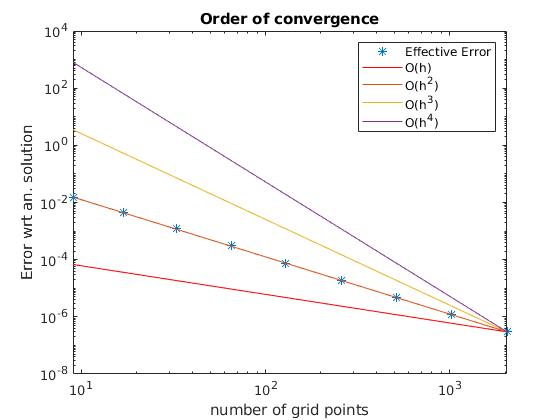
\includegraphics[width=0.8\textwidth]{OrderConst.jpg}
	  \caption{Order of convergence depending on the number of grid points}
	  \label{fig:OrderConst}
\end{figure}

\section{Implementation}
Now we describe the code. First of all we set the constants, the potential and the space interval. We need to find the energy levels where the resonance is. We will use a space uniform mesh to approximate the probability density function for fixed level of energy using the method described previously after the nondimensionalization. We set an energy uniform mesh, we find the approximate solutions for the different energy  levels and we compute the transmission coefficients for these energy values. Then we refine uniformly the mesh used (e.g. dividing by $2$ the length of the energy subintervals because we don't want to increase too much the computational cost) and we compute the new approximate solutions and transmission coefficients.  Now we need to locate the energy regions where the resonance could be. We compare the transmission coefficients of the actual energy mesh and the previous one. In the previous mesh we have less values of energy for which the transmission coefficient is computed, so we need more values for the previous transmission coefficients. We used a linear interpolation to compute the transmission coefficient for the missing values of energy. The transmission coefficient is a number between $0$ and $1$ therefore the difference of the transmission coefficients could be very small, so we computed the relative error between the logarithms. For every energy value of the current mesh when the relative error is greater than a fixed tolerance we store the energy point. These levels of energy identify the regions where we need to refine the energy mesh. We have to separate the regions to detect those where the error is too high and we need to refine the energy mesh and to avoid to refine the energy mesh where it is useless. We calculated the variation of the logarithm of the actual transmission coefficient and we studied it on the energy levels found previously. When we have a peak the variation before it is positive and then negative. The region of one peak is identified by the levels of energy where the variation first is positive (to find the part of the region on the left of the peak) and then is negative (to find the part of the region on the right of the peak). When the variation from negative becomes positive the region is over. For every region we compute the error on the logarithm of the transmission coefficient and, if it is greater than another fixed tolerance, we need to refine the energy mesh in that region (e.g. dividing by $5$ or $10$ the energy step). Now we have constructed a new mesh that becomes the current one and the one before the refinement becomes the previous one and we repeat this procedure until a maximum number of iteration is reached or the error is below a fixed tolerance.\\
In the next figures we will study the behavior of the transmission coefficient and the refinement of the energy mesh of two different potentials, one on the left side with two barriers and the other one on the right side with five barriers.

\begin{figure}[h!]
\subfigure[2 barriers potential]
{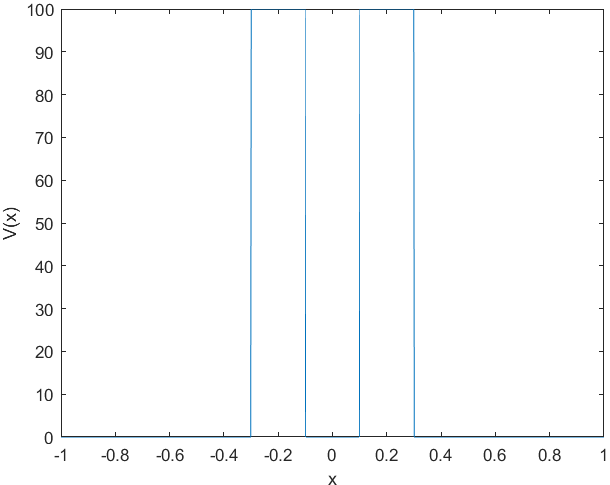
\includegraphics[width=0.48\textwidth]{2barriers.png}} \quad
\subfigure[5 barriers potential]
{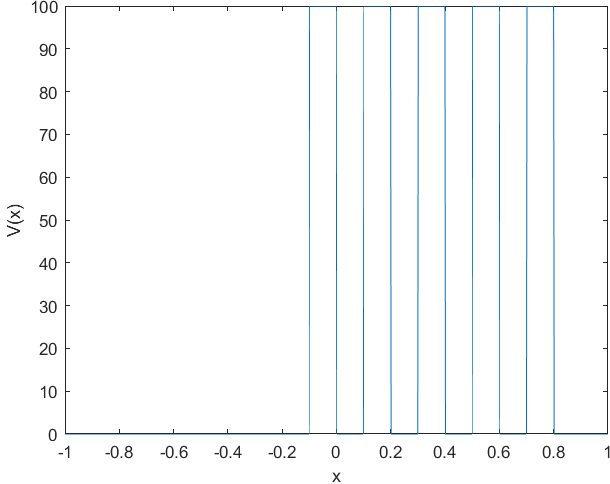
\includegraphics[width=0.48\textwidth]{5barriers.png}}
\caption{Potentials} \label{fig:potential}
\end{figure} 

\begin{figure}[h!]
\subfigure[2 barriers potential]
{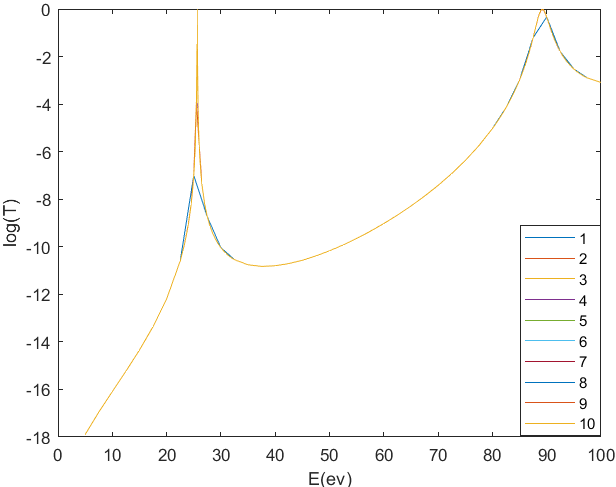
\includegraphics[width=0.48\textwidth]{Tit2.png}} \quad
\subfigure[5 barriers potential]
{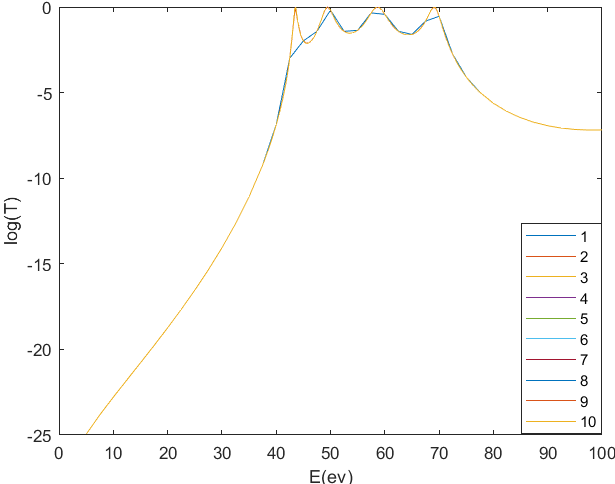
\includegraphics[width=0.48\textwidth]{Tit5.png}}
\caption{Approximations of the transmission coefficient at different iterations} \label{fig:logTransmissionCoefficient}
\end{figure}

\begin{figure}[h!]
\subfigure[2 barriers potential]
{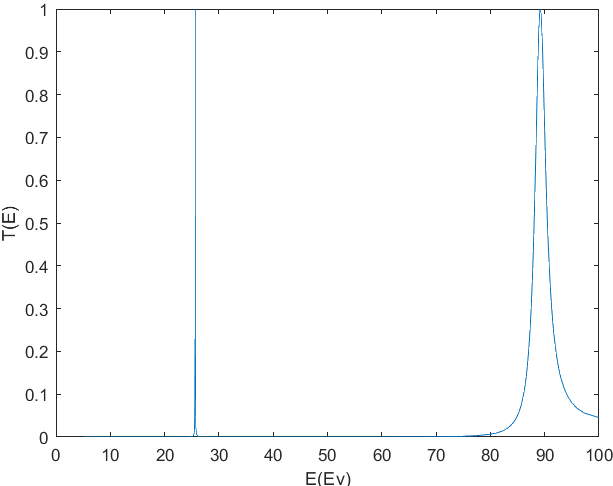
\includegraphics[width=0.48\textwidth]{T2.png}} \quad
\subfigure[5 barriers potential]
{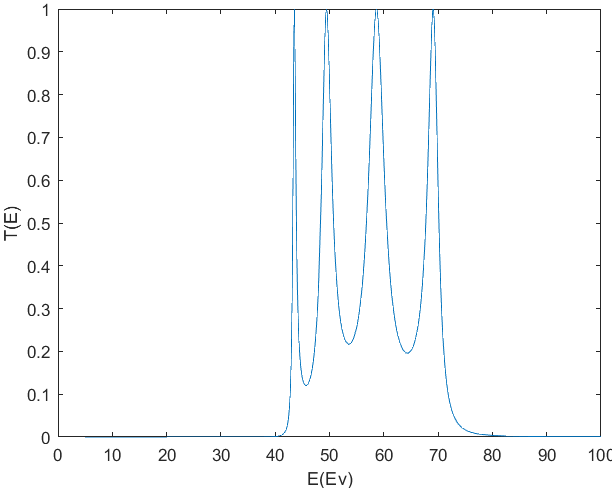
\includegraphics[width=0.48\textwidth]{T5.png}}
\caption{Transmission coefficient}\label{fig:transmissionCoefficient}
\end{figure}

In Figure \ref {fig:logTransmissionCoefficient} there are the approximations of the logarithm of the transmission coefficients after some iterations. We note that there are two peaks for the left potential and four for the right one. In Figure \ref {fig:transmissionCoefficient} there are the approximations of the transmission coefficients.

\begin{figure}[h!]
\subfigure[2 barriers potential]
{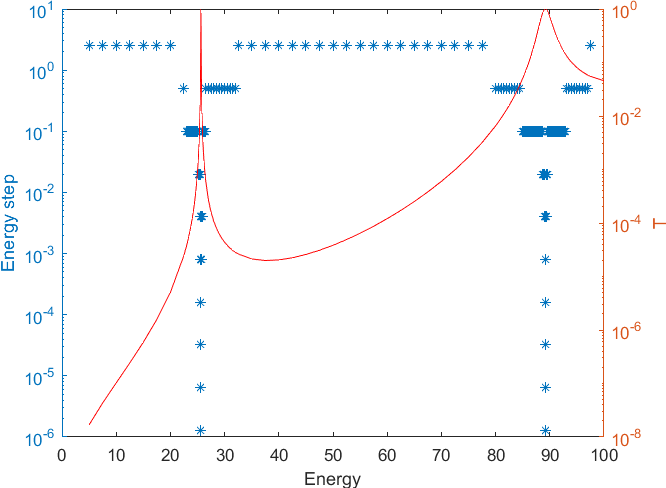
\includegraphics[width=0.48\textwidth]{2refinement.png}} \quad
\subfigure[5 barriers potential]
{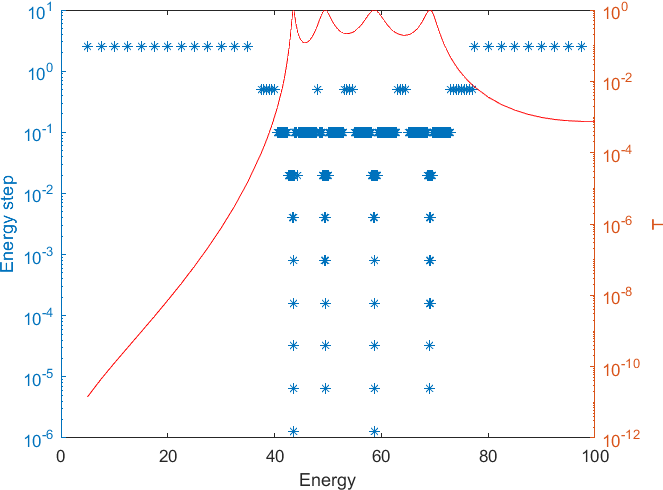
\includegraphics[width=0.48\textwidth]{5refinement.png}}
\caption{Mesh refinement and transmission coefficient} \label{fig:refinement}
\end{figure}

In Figure \ref {fig:refinement} we have on the left of the graphics the scale for the energy step represented with stars, on the right the scale for the transmission coefficient. We notice that near the peaks the energy step becomes really small.




\section{Possible improvement:  Galerkin approach}


Since the regularity of $\var$ strongly depends on the regularity of the potential $V(x)$, with a finite difference approach one lose the second order approximation. Indeed, with piece-wise constant potential we have no more second order approximation. This observation leads to a Galerkin approach, requiring the solution $\var(x)$ to be less smooth than before. 

Denoting with $H^1(0,1)$ the Sobolev space $W^{1,2}(0,1)$, as usual we take a $v \in H^1(0,1)$, multiply the equations by $v$ and integrate by parts:


\[
\int_{0}^{1} \var ''(x) v(x)  \text{dx} + 2 \int_0^1 (E-V(x))\var (x) v(x) \text{dx} =0, \quad v \in H^1(0,1)
\]



\[
[\var '(x) v(x)]_{0}^{1} - \int_{0}^{1} \var '(x) v'(x)  \text{dx}+ 2 \int_0^1 (E-V(x))\var (x) v(x) \text{dx} =0, \quad v \in H^1(0,1)
\]

Recalling that we have Robin boundary conditions, then in the weak formulation we will have terms proportional to $\var $. Using the fact that $\var'(0)=2 \bold{i} k - \bold{i} k \var(0)$ and $\var'(1)=\bold{i}k_2 \var(1)$ then the weak formulation is to find $u \in H^1(0,1)$ such that the following identity:

\[ 
\bold{i} k_2 \var(1)v(1) + \bold{i} k \var(0) v(0) -2 \bold{i}k v(0) - \int_0^1 \var' v' \text{dx} + 2 \int_0^1(E-V(x)) \var v \text{dx} = 2 \bold{i}k, 	\quad (\star)
\]

holds for every $v \in H^1(0,1)$.

In order to solve it, we restrict to a proper finite dimensional subspace $X_h$ of $H^1$, made by piecewise linear functions, i.e. $X_h= \{ w \in H^1(0,1): w_{|[x_i,x_{i+1}]} \in \mathbb{P}([x_i,x_{i+1}])\}$. A basis of this space $X_h$ is given by the ``hat functions'' $w(x)$ and therefore we have to search for $\var_h \in X_h$ such that $(\star)$ holds for every $v \in X_h$. In particular, we have

\begin{equation}
\label{eqn:fem}
\var_h(x)=\sum_{i=1}^{N} (\var_h)_j w_j(x)
\end{equation}

and the discrete problem is therefore to find $\var_h \in X_h$ s.t.

\[
-\int_0^1  \sum_j (\var_h)_j w_j'(x) w_i'(x) \text{dx} + 2 \int_0^1 (E-V(x)) \sum_j (\var_h)_j w_j(x) w_i(x) \text{dx} + \bold{i}k (\var_h)_1 w_{1}^{2}(0) + i k_2 (\var_h)_N w_N^{2}(1)= 2 \bold{i} k
\]

for $1\leq i \leq N$ 




At this point one can assembly the \emph{stiffness} matrix $A$, the ``load'' vector $\boldsymbol{b}$ and solve the linear system \[
A \boldsymbol{\var}_h= \bold{b}\]
Note that the solution of the linear system will give the coefficients $\var_h$ of  \eqref{eqn:fem}, not the values of $\var$ at the nodes as in the finite difference approach.





















\section{Validation}
\subsection{Variating the potential}
Until now, we have tested identical potential barriers with the same value and ratio of width barrier/well. An important test now is to check if the optimization depends on the form of the potential. In Figure \ref {fig:modified_potentials} we show the tested modified potentials and in Figure \ref{fig:modified_1} and Figure \ref{fig:modified_2} the results.

\begin{figure}[H]
\centering
		\subfigure[Modified 4 barrier potential]{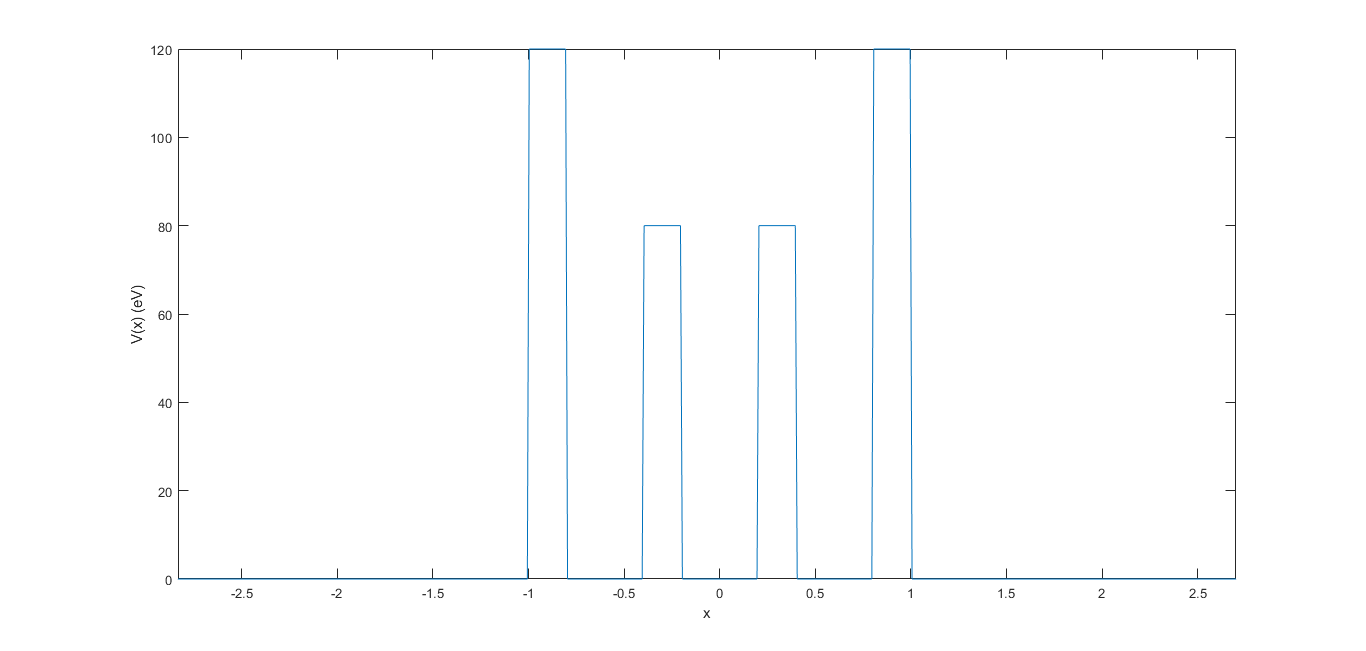
\includegraphics[width=0.48\linewidth]{4mbarriers.png}}
		\subfigure[Modified 3 barrier potential]{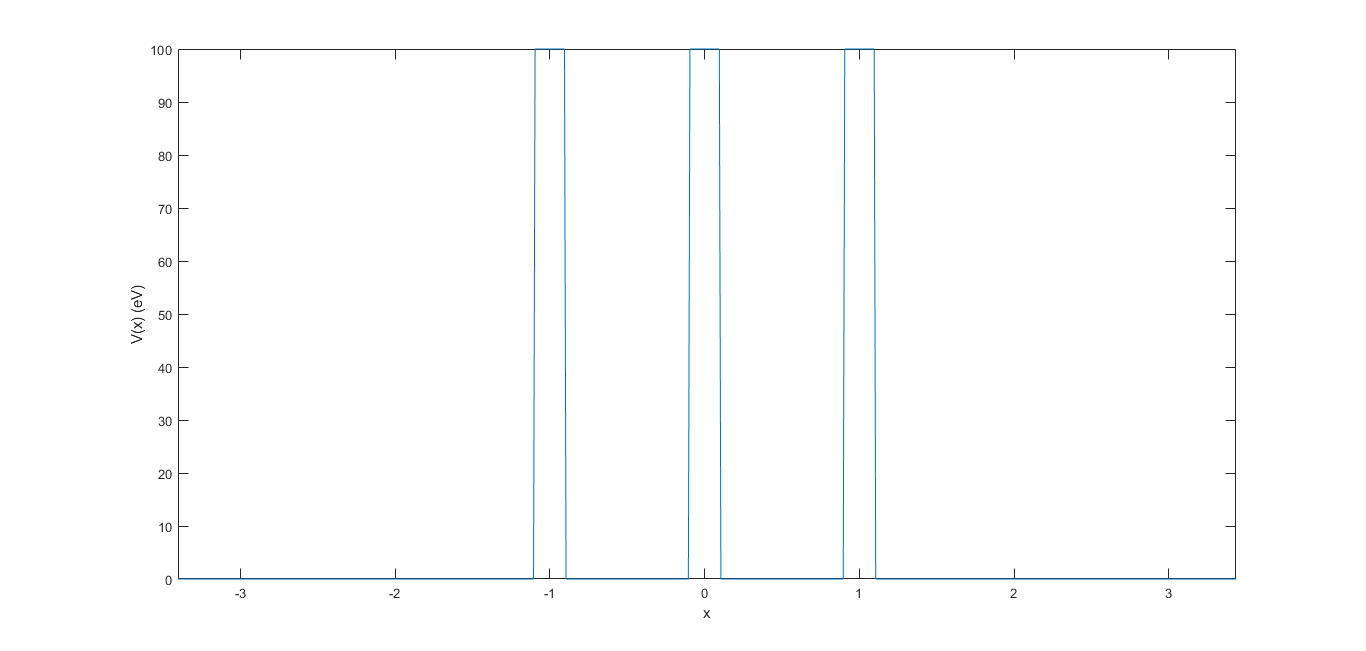
\includegraphics[width=0.48\linewidth]{3lbarriers.png}}
	\caption{Tested modified potentials. On one hand we tried modifying the heights of the intermediate potentials and on the other we increased the weidth of the quantum wells, with 3 barriers.} 
	\label{fig:modified_potentials}
\end{figure}

\begin{figure}[H]
\centering
		\subfigure[$log(T)$ for the baseline code]{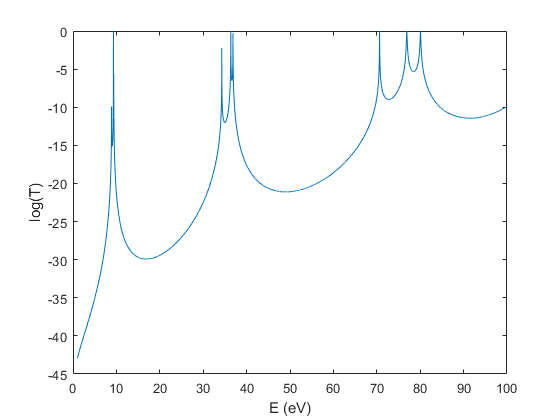
\includegraphics[width=0.45\linewidth]{logT_4barr_nop.png}}
		\subfigure[$log(T)$ for the optimized code]{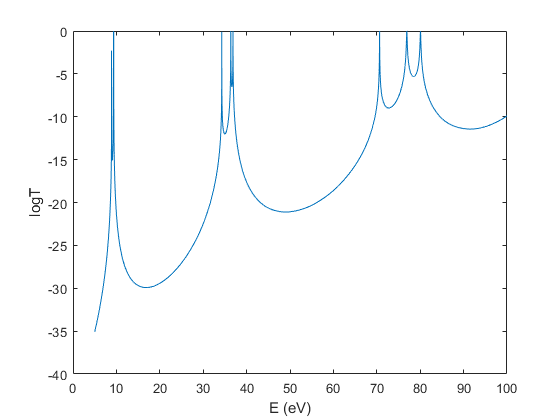
\includegraphics[width=0.45\linewidth]{logT_4barr_sip.png}}
	\caption{Test of the optimized code for the modified 4 barriers potential} 
	\label{fig:modified_1}
\end{figure}

\begin{figure}[H]
\centering
		\subfigure[$log(T)$ for the baseline code]{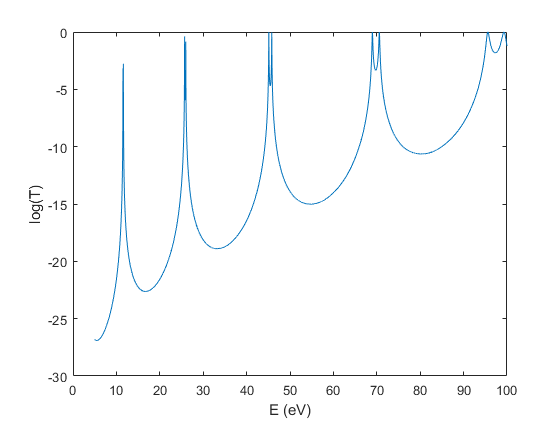
\includegraphics[width=0.45\linewidth]{logT_3barr_nop.png}}
		\subfigure[$log(T)$ for the optimized code]{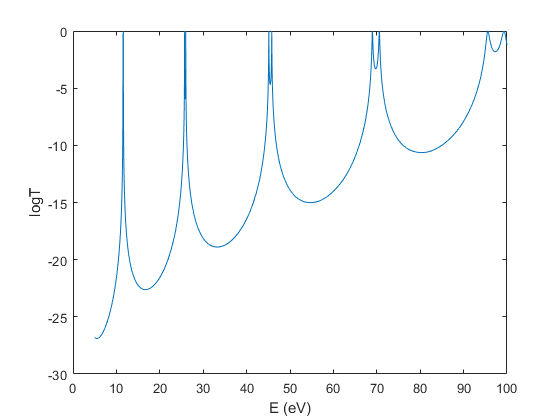
\includegraphics[width=0.45\linewidth]{logT_3barr_sip.png}}
	\caption{Test of the optimized code for the modified 3 barriers potential} 
	\label{fig:modified_2}
\end{figure}	

From the figures we can appreciate that our optimization passed correctly the presented test, and also we observed that this modifications on the potential produced significant differences on the position of the transmission coefficient's peaks. What's more, from this tests we extracted some remarking features of the model that can be of high interest when building the devices. For instance, we observe that a direct relation between the number of quantum wells and the number of peaks into which the transmission peaks of the 3-barrier is splitted (this effect is better shown in Figure \ref {fig:peak_split}). When modifying the height of the intermediate barriers we also observed that the apparent symmetry into which the peaks are splitted is broken, as Figure \ref {fig:modified_1} shows. On the other hand, when increasing the width of the wells, the number of energy states inside the well is also increased, allowing for more resonant transmission peaks. This effect is already shown in Figure \ref {fig:modified_2} and is exaggerated in Figure \ref {fig:peak_increase}.

\begin{figure}[H]
\centering
		\subfigure[Barriers=3]{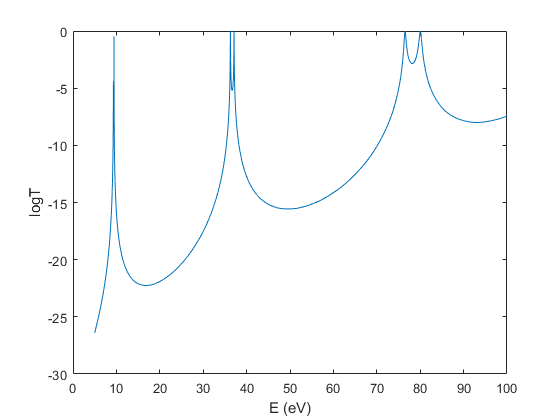
\includegraphics[width=0.45\linewidth]{logT_3barr_peaks.png}}
		\subfigure[Barriers=5 (zoomed)]{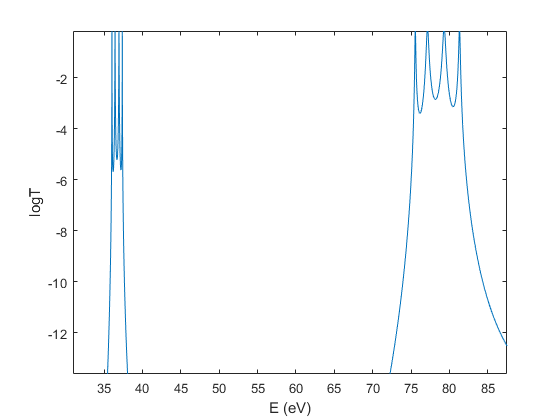
\includegraphics[width=0.45\linewidth]{logT_5barr_peaks.png}}
	\caption{Illustration of how increasing the number of barriers splits the peaks in the same amount.} 
	\label{fig:peak_split}
\end{figure}

\begin{figure}[H]
\centering
		\subfigure[Well width =$0.2$]{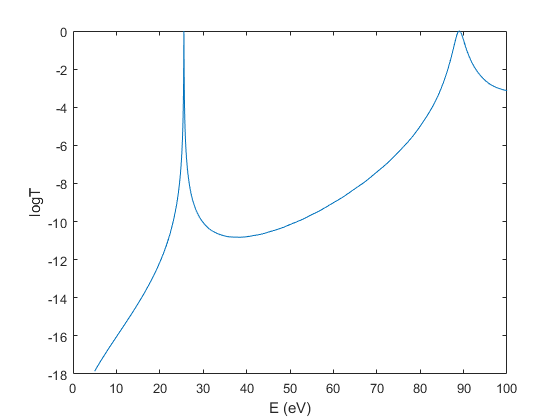
\includegraphics[width=0.45\linewidth]{energies2_02.png}}
		\subfigure[Well width=$0.8$]{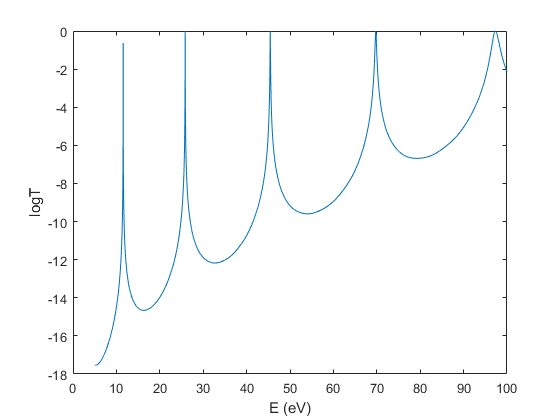
\includegraphics[width=0.45\linewidth]{energies2_08.png}}
	\caption{Illustration of how increasing the width of the wells allow for more energy resonances.} 
	\label{fig:peak_increase}
\end{figure}

\section{Conclusions}

Other possible improvements can be made changing the stopping condition of the cycle in the implementation. With our code the number of iteration always reaches its maximum, but we would like that sometimes it stops before.\\
Every cycle we compute the solutions for every energy level of the new mesh, but for many of these levels it is useless because we have already computed the solution. At every iterations we could  keep track of the solutions computed and avoid to recompute them and make the implementation quicker.\\
As described before, the numerical solution itself could be improved by using, for instance, a Galerkin approach.\\
We can also change our method to find the regions of energy refinement looking at the probability density after the first barrier of the potential. If the value of the probability is big enough something has passed through the barrier and we have to refine the energy mesh there.\\
Eventually we can study the behavior of the solution as time goes by computing the exact time dependent solution (it is really easy).   


\section{Job splitting}

Most of us did not have a sufficient the physical background, so we had to split the job somehow. Some of us were more practical from a numerical point of view, while others were more confident with the physics and the analysis behind the equation, so we decided to split our group in essentially two subgroups. For instance, in order to check the numerical results and see if they were reliable with the theory, we had to discuss together. We spent the first days familiarizing with the analytical and numerical solution of the equation itself, especially with the "transparent boundary conditions", since all of us were not familiar with them. After this, we checked if our numerical solution agreed with the analytical one. The remaining days we worked to the refinement of the energy, which was the main topic of the project. The time, of course, was not enough to make an optimized work, since lots of features can be improved a lot, as highlighted above.


\newpage
%\thispagestyle{empty}
\addcontentsline{toc}{section}{REFERENCES}

\bibliographystyle{authoryear} % for Harvard (author-year) citation style
% to insert bibliography create a .bib file with all the entries
% For citing with natbib use \citet and \citep commands
% \citet cites as a part of the sentence in form Author (year)
% \citep cites in parentheses in form (Author, year)

% For numerical citation style package natbib is not required
% and the bibliography itself can be created without using external .bib file
% as follows:



\begin{thebibliography}{99}
\bibitem{resonantpaper}
``Coaxial Nanowire Resonant Tunneling Diodes from non-polar AlN/GaN on Silicon'', Carnevale, S.D. et al.; Appl. Phys. lett. 100, 142115 (2012) \\
\href{https://arxiv.org/abs/1202.6052}{\footnotesize https://arxiv.org/abs/1202.6052}

\bibitem{bc}
%ASK CLEMENT FOR THE AUTHORS/ARTICLE !

\bibitem{IncidentWave}
Incident wave definition\\
\href{https://uk.farnell.com/incident-wave-definition}{\footnotesize https://uk.farnell.com/incident-wave-definition}

\bibitem{wikiTransmCoeff}
Transmission coefficient\\
\href{https://en.wikipedia.org/wiki/Transmission\_coefficient}{\footnotesize https://en.wikipedia.org/wiki/Transmission\_coefficient} 

\bibitem{ConservationLaw}
Conservation of probability\\
\href{https://quantummechanics.ucsd.edu/ph130a/130\_notes/node127.html}{\footnotesize https://quantummechanics.ucsd.edu/ph130a/130\_notes/node127.html}

\bibitem{wikiProbCurrent}
Probability current \\
\href{https://en.wikipedia.org/wiki/Probability\_current}{\footnotesize https://en.wikipedia.org/wiki/Probability\_current}

\bibitem{wikiStatState}
Stationary state \\
\href{https://en.wikipedia.org/wiki/Stationary\_state}{ \footnotesize https://en.wikipedia.org/wiki/Stationary\_state}
\end{thebibliography}
% Then use \cite{marker} to cite the references in the text.



\end{document}
